\chapter{Optimierung der Ausführungsparameter}

Die Ausführungszeit der in den vorherigen Kapiteln vorgestellten Algorithmen wird stark durch unterschiedliche Parameter beeinflusst.
Den größten Einfluss nimmt dabei die Art des Datensatzes, also wie viele Matches er enthält, wie lang die enthaltenen Zeichenketten sind, wie viele Strings im Datensatz vorhanden sind und wie die Matches darin verteilt sind.
Wie sehr unterschiedliche Datensätze die Ausführungszeit beeinflussen soll in Kapitel \ref{sec:equals_evaluation} untersucht werden.

Neben dem Aussehen des Datensatzes gibt es noch Parameter, die bei der Ausführung des Algorithmus der GPU übermittelt werden und dort ebenfalls einen starken Einfluss auf die Laufzeit nehmen können.
Diese Parameter bestehen wie in Kapitel \ref{sec:cuda_scheduling} beschrieben in der Anzahl der Threads pro Block (\emph{Block Size}) und der Anzahl der Blöcke im Grid (\emph{Grid Size}).
Aus den Parametern setzt sich die \emph{Grid-Konfiguration} zusammen, welche durch das Ausprobieren unterschiedlicher Werte optimiert werden kann.

\begin{figure}[ht]
	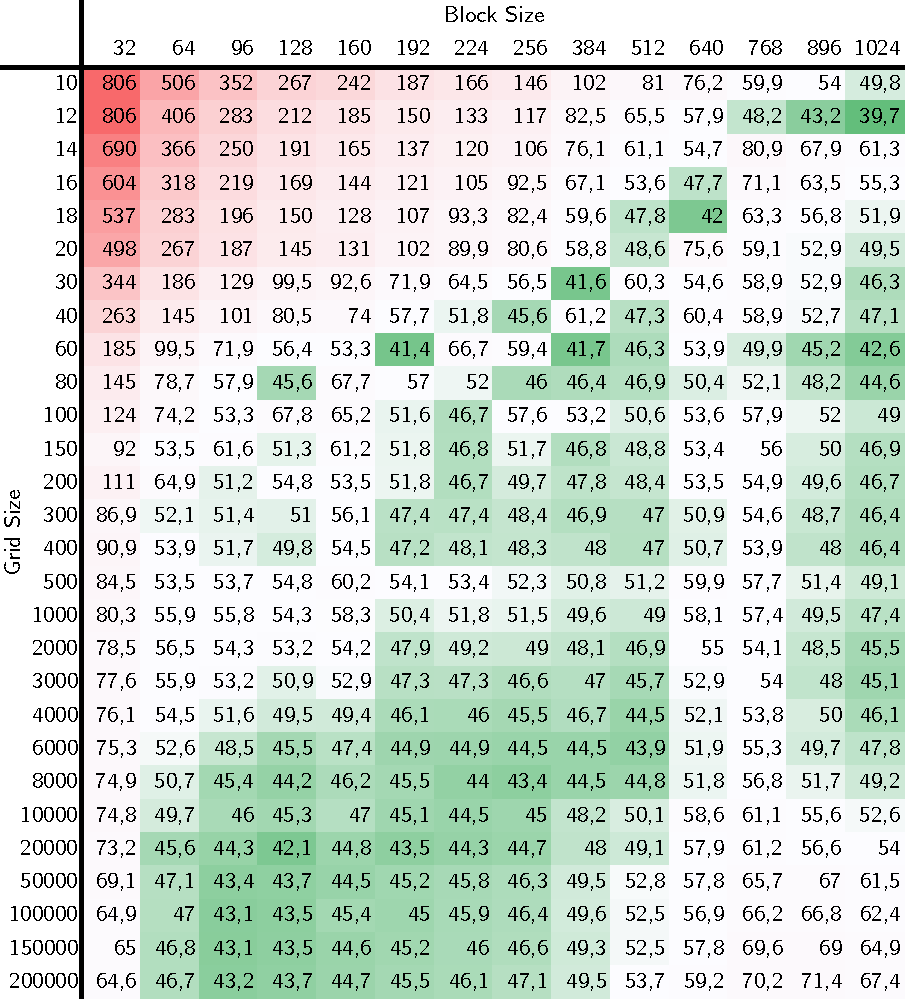
\includegraphics[]{bilder/parameter025.pdf}
	\caption{Laufzeit des naiven String-Vergleichsalgorithmus in ms für den Type-Datensatz mit einer Selektivität von 0.25\% unter Verwendung unterschiedlicher Grid-Konfigurationen}
	\label{gpu_architecture}
\end{figure}

Um dieses Vorgehen zu veranschaulichen, soll anhand eines Beispiels gezeigt werden, wie eine möglichst optimale Grid-Konfiguration gefunden werden kann und wie unterschiedliche Konfigurationen einen Einfluss auf die Laufzeit nehmen.
Abbildung \ref{gpu_architecture} zeigt dazu die Laufzeit für den String-Vergleichsalgorithmus in Millisekunden, welcher für unterschiedliche Grid-Konfigurationen auf dem in Kapitel \ref{sec:equals_evaluation_workloads} vorgestellten Type-Datensatz mit einer Selektivität von 0.25\% ausgeführt wurde.
Besonders hohe Laufzeiten sind dabei in rot und besonders niedrige Laufzeiten in grün eingefärbt.

Es fällt auf, dass eine niedrige Block Size in Kombination mit einer niedrigen Grid Size zu einer hohen Laufzeit führt.
Außerdem gibt es bei einer Grid Size von unter 100 einige Kombinationen, die besonders geringe Laufzeiten aufweisen, allerdings von weniger guten Konfigurationen umgeben sind.
Mit einer Grid Size zwischen 2.000 und 200.000 in Verbindung mit einer Block Size zwischen 64 und 512 werden generell ordentliche Laufzeiten erzielt.
Wird allerdings eine Block Size über 512 gewählt, nimmt die Leistungsfähigkeit des Systems wieder ab.

Generell ist die Analyse eines solchen Ergebnisses schwierig, da die Grid-Konfiguration Einfluss auf unterschiedlichste Bereiche der GPU nimmt und der CUDA-Optimierer einige Effekte erfolgreich versteckt.
Die hohe Laufzeit des Algorithmus bei einer geringen Anzahl von Threads ist dadurch zu erklären, dass zunächst gar nicht alle Kerne der GPU ausgelastet sind, weil nicht genügend Warps für die Anzahl der SM vorhanden sind.
Eine steigende Anzahl von Threads führt zwar dazu, dass alle Kerne ausgelastet sind, allerdings können bei Speicherzugriffen nicht genügend Warps vom Scheduler ausgetauscht werden, sodass wie in Kapitel \ref{sec:cuda_scheduling} beschrieben die Latenz der Speicherzugriffe erfolgreich versteckt werden könnte.
In dem zuvor beschriebenen Bereich, in dem ordentliche Laufzeiten erzielt werden, steht eine ausreichende Anzahl von Threads zur Verfügung, um eventuelle Latenzen zu verstecken und somit die GPU bestmöglich auszulasten.
Wie der Anstieg der Laufzeiten bei einer Block Size von über 512 zu begründen ist, wird hier leider nicht klar.

Für die Verwendung des Algorithmus sollte im Allgemeinen eine Grid-Konfiguration aus dem Bereich gewählt werden, welcher eine durchweg ordentliche Performanz erzielt.
Dadurch ist die Wahrscheinlichkeit hoch, dass eine Konfiguration gewählt wird, mit der eine Laufzeit erreicht wird, welche bis auf eine kleinere Abweichung dem Optimum entspricht.
Die Position des Bereichs ändert sich für unterschiedliche Selektivitäten des Datensatzes nur geringfügig, wie in zahlreichen Tests untersucht wurde und beispielhaft in Anhang \ref{apx:parameter64} für eine Selektivität von 64\% analog zu Abbildung \ref{gpu_architecture} dargestellt wird.
Aus diesem Grund kann die Grid-Konfiguration schon vor der Ausführung bestimmt werden und eine nah am Maximum liegende Leistungsfähigkeit erzielt werden.
Bei den Leistungsmessungen in den folgenden Kapiteln sollte sich allerdings nicht darauf verlassen werden, dass durch diese Heuristik ein nahezu optimaler Wert gefunden wird, weshalb für die Tests jeweils das Optimum aus einer Auswahl von Grid-Konfigurationen bestimmt wird.
Dazu werden alle Konfigurationen mit einer Grid Size von \{1.000, 2.000, 3.000, 4.000, 6.000, 8.000, 10.000, 20.000, 50.000, 100.000, 150.000, 200.000\} und einer Block Size von \{32, 64, 96, 128, 160, 192, 224, 256, 384, 512, 640, 768\} überprüft und das Optimum der Messungen für die Auswertung der aufgestellten Statistiken gewählt.